\section{The languages of the compiler}
When creating a compiler there are three languages of relevance, as seen in the tombstone diagram\ref{fig:TStoneExample}.

\begin{figure}[H]
	\centering
	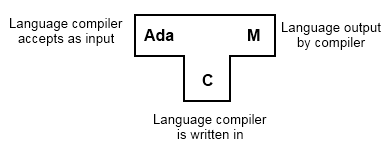
\includegraphics[width=\textwidth/2+\textwidth/4]{4.Solution/images/T-diagram.png}
	\caption{
		Example of Tombstone diagram showcasing an example of three languages for a given compiler\cite{TStoneWiki}.
	}
	\label{fig:TStoneExample}
\end{figure}
In the case of the HCL compiler the three languages are as follows:

\begin{enumerate}
\item input: \textbf{HCL} \\
\item output: \textbf{C++/C} \\
\item compiler: \textbf{Kotlin} \\
\end{enumerate}

\subsection{Language of the compiler}
The compiler was written in Kotlin\cite{KotlinWebsite}, a new programming language that compiles to both the JVM, javascript and LLVM. 
The compiler is compiled to JVM because this grants access to all of the java ecosystem libraries, which in turn makes the JVM the most used target of kotlin.
The choice to use kotlin was based on a number of factors.
The group wanted to experiment with using a language they had no prior experience with for the duration of the project, but because of time limitations, a new language had to adhere to already known paradigms.
The group knew C\# and a bit of Java, however as the HCL language has a lot of functional features, it was deemed important that the group became comfortable with a language that, at the very least was multi paradigm.
Kotlin is inspired by both C\# and java and have a fairly similar syntax to that of those, which made it easier to learn from the perspective of the group.
However it is still possible to write methods that is utilizes a functional domain.

This grants the developer a large amount of possibilities, while still being relatively easy to learn.
A disadvantage could be that low-level languages might have faster executing time. 
However, as HCL is built with the Arduino architecture in mind, it is not possible to create vast programs due to hardware limitations
Therefore execution time of the compiler will never really affect the end user, as the difference should not be noticeable.

\subsection{Output language of the compiler}
The group initially wanted to compile to assembly, primarily for educational purposes, however as the initial brainstorming took place, the group quickly realized that they wanted a big set of possibilities, which would waste a lot of development time on code generation. 
In order to save time, the group agreed on compiling to C++, the language that Arduino software is normally written in.
When writing code in the Arduino IDE, it gives access to predefined methods for interacting with I/O devices.
It then runs the code through a C/C++ compiler\cite{ArFAQ}.

However, the standard library is not accessible in the Arduino language, which means that dynamic lists, vectors, and other similar constructs are not accessible.
Therefore it was required that the development team of HCL would implement some of these constructs manually.
This is still a lot easier than compiling to assembly directly. 
The compilation process, with this is mind, will essentially be: Compile to the Arduino-subset of C++, and then let the Arduino software generate assembly code from the code generated by the HCL compiler.
This is shown in detail in figure \ref{fig:HCLTStone}.


\begin{figure}[H]
	\centering
		\begin{tikzpicture}
		\begin{tombstonediagram}
		\compiler{cmp}{H}{C++}{JVM}{}
		\program[anchor=prg-2-2.north east]{prg}{Source}{H}{at (cmp-1-1.north west)}
		\interpreter{int}{JVM}{x86}{at (cmp-2-2.south west)}
		\program{prgo}{Source}{C++}{at (cmp-1-3.north east)}
		\machine{mac}{x86}{at (int-2-1.south west)}
		\compiler{cmp2}{C++}{MC}{x86}{at (prgo-1-2.south east)}
		\machine{mac2}{x86}{at (cmp2-2-2.south west)}
		\program{prgo2}{Source}{MC}{at (cmp2-1-3.north east)}
		\end{tombstonediagram}
		\end{tikzpicture}
	\caption{
		Tombstone diagram for the HCL to Arduino compilation.
		H is HCL, MC is Arduino machine code.
		The HCL to C++ compiler runs on the JVM as Kotlin runs on the JVM.
	}
	\label{fig:HCLTStone}
\end{figure}


